\documentclass{article}

\usepackage{caption}
\usepackage{subcaption}
\usepackage{amsmath}

\usepackage{arxiv}

\usepackage[utf8]{inputenc} % allow utf-8 input
\usepackage[T1]{fontenc}    % use 8-bit T1 fonts
\usepackage{hyperref}       % hyperlinks
\usepackage{url}            % simple URL typesetting
\usepackage{booktabs}       % professional-quality tables
\usepackage{amsfonts}       % blackboard math symbols
\usepackage{nicefrac}       % compact symbols for 1/2, etc.
\usepackage{microtype}      % microtypography
\usepackage{lipsum}
\usepackage{graphicx}

\usepackage{algorithm2e}
\usepackage{authblk}
%\usepackage{bbding}
\usepackage{multirow}
\usepackage{makecell, tablefootnote, longtable}

%\usepackage{multicol}
%\setlength{\columnsep}{20pt}

\usepackage[backend=biber]{biblatex}
\addbibresource{refs.bib}

\graphicspath{ {./fig/} }

\usepackage{tikz}
\usetikzlibrary{arrows.meta, bending, positioning}

\hypersetup{colorlinks=true,linkcolor=blue,filecolor=magenta,urlcolor=cyan}
\newcommand{\map}{\mathop{\bigoplus}\limits}
\newcommand{\txtop}[1]{\mathop{\mathtt{#1}}\limits}

\newcommand{\expr}{\txtop{expression}}

\newcommand{\fn}{\txtop{function}}
\newcommand{\tanhl}{\txtop{tanh}}
\newcommand{\linear}{\txtop{linear}}
\newcommand{\sigmoid}{\txtop{sigmoid}}
\newcommand{\argmin}{\txtop{argmin}}
\newcommand{\einsum}{\txtop{einsum}}
\newcommand{\ntos}{\txtop{noise2self}}
\newcommand{\leiden}{\txtop{leiden}}
\newcommand{\relu}{\txtop{ReLU}}

\newcommand{\encoder}{\txtop{encoder}}
\newcommand{\decoder}{\txtop{decoder}}
\newcommand{\classifier}{\txtop{classifier}}
\newcommand{\partitioner}{\txtop{partitioner}}
\newcommand{\Conv}{\txtop{Conv}}
\newcommand{\ConvT}{\txtop{Conv^\top}}

\newcommand{\mathSAE}{\txtop{SAE}}
\newcommand{\mathSAET}{\txtop{SAE^\top}}

\newcommand{\mathWAK}{\txtop{WAK}}
\newcommand{\mathPWAK}{\txtop{PWAK}}
\newcommand{\mathDEWAKSS}{\txtop{DEWAKSS}}
\newcommand{\mathPart}{\txtop{Partitioner}}
\newcommand{\mathDeePWAK}{\txtop{DeePWAK}}
\newcommand{\mathDeePWAKBlock}{\txtop{DeePWAKBlock}}

\SetKwProg{Fn}{Function}{}{end}
\SetKwProg{Dat}{Data}{}{end}

\SetKwInOut{Hyper}{Hyperparameters}

\SetKwFunction{softmax}{softmax}
\SetKwFunction{MSE}{MSE}
\SetKwFunction{transpose}{transpose}
\SetKwFunction{matmul}{matmul}
\SetKwFunction{eucl}{euclidean}
\SetKwFunction{pca}{pca}
\SetKwFunction{knn}{knn}

\SetKwFunction{sample}{sample}
\SetKwFunction{loss}{loss}
\SetKwFunction{train}{train}

\SetKwFunction{WAK}{WAK}
\SetKwFunction{PWAK}{PWAK}
\SetKwFunction{DEWAKSS}{DEWAKSS}
\SetKwFunction{DeePWAKBlock}{DeePWAKBlock}
\SetKwFunction{DeePWAK}{DeePWAK}

\SetKwFunction{Type}{Type}
\SetKwFunction{List}{List}
\SetKwFunction{Arch}{Arch}
\SetKwFunction{Params}{Params}
\SetKwFunction{Model}{Model}
\SetKwFunction{Linear}{Linear}
\SetKwFunction{Partitioner}{Partitioner}

%\newcommand{\subhead}[1]{{\Large #1 \vspace{2ex}}}
\newcommand{\secsubhead}[1]{{\itshape (#1) \vspace{2ex}}}



\date{\today}

%\title{Are Data Singular?}
\title{Finding an Interpretable Feature Basis with Self-Supervised Classification}
%\title{Finding an Interpretable Basis with Cluster-Embedding Decomposition}
%\title{Sparse Autoencoders, Clustering, and Natural Abstractions}
%\title{Can Sparse Autoencoders Identify Natural Abstractions?}
\subtitle{Aggregating data into maximum entropy clusters produces sparse and interpretable features 
even without a sparcity penalty}

\author[1]{Keira Wiechecki}
\affil[1]{Center for Genomics \& Systems Biology, New York University,
  \texttt{kaw504@nyu.edu}}

\begin{document}

\maketitle


\begin{abstract}
I identify two powerful but somewhat obscure unsupervised learning principles with neglected potential
to advance interpretability research.
%The first is self-supervised denoising as a loss functio:
%for a large class of denoising functions, it is possible to minimize loss using only unlabeled,
%noisy data.
The first is causal emergence:
a high entropy graph can be aggregated into a low entropy representation.
The second is self-supervised denoising:
graph aggregation can be expressed as a denoising function which can be optimized with no prior knowledge.  
I present a modified version of a sparse autoencoder based on these principles.
%  I present a formulation of clustering as an unsupervised classification problem.
%  I present a novel deep clustering architecture using an unsupervised classifier (UC) to find a denoising kernel.
%  Training the UC in parallel with a sparse autoencoder (SAE) discovers features that best capture variation between clusters.
%  I term this cluster-embedding ($KE$) decomposition.
%In this proposal, I introduce a novel method for analyzing the feature space of a model combining clustering and denoising,
%which I term cluster-embedding ($KE$) decomposition.
%By treating clustering as an unsupervised classification problem, 
%we can obtain a denoising diffusion kernel based on the probability of sample pairs being in the same cluster.
%By training the unsupervised classifier in parallel with a sparse autoencoder,
%we can identify ``basis features'' which distinguish maximum entropy clusters.
  %Remarkably, the aggregate clusters obtained from the information bottleneck of an MNIST classifier
  %have nearly 1-to-1 correspondence to the model's latent representation.
  Preliminary experiments on a toy model of superposition suggest this method produces a sparser, 
  more interpretable features than a na\"ive SAE. 
In the short term, I plan to assess whether this method can detect concept formation, validate these results across a representative set of toy models,
  and determine a rigorous metric for comparing the interpretability of features.
  In the extension phase I would like to scale this approach to GPT-2.
  
  %I propose $KE$ decomposition deserves further study as a potentially powerful and versatile interpretability tool.
  
%  I further propose that the feature space can be decomposed into two subspaces with intuitive interpretations:
%  a cluster space and an embedding space.
%  This approach suggests a model's latent ontology can be derived using a paired encoder and unsupervised classifier.
  
\end{abstract}

%\begin{multicols}{2}

\section{Threat Model}

We don't currently know how to specify a \hyperlink{https://arbital.com/p/diamond_maximizer/}{robust goal for a model}.
Because goal space is large, we should expect
\hyperlink{https://www.lesswrong.com/s/r9tYkB2a8Fp4DN8yB/p/FkgsxrGf3QxhfLWHG}{goal misgeneralization as the default outcome}
\footnote{The most straightforward path to doom is for a goal-driven superintelligence to seize power to prevent its optimization target from being changed.
In slow takeoff or multipolar scenarios, there is also a ``decoherence'' risk, 
where comparably weak specialist optimizers disempower humanity without any coherent strategy.
Consider for instance superpersuaders which fall short of superintelligence.
A viral chatbot might have very simple objectives to optimize engagement and distribution of itself.
While such a scenario would be an especially 
\hyperlink{https://www.lesswrong.com/posts/mSF4KTxAGRG3EHmhb/ai-x-risk-approximately-ordered-by-embarrassment}{undignified} 
end for humanity,
it broadly fits with both natural language being much easier than anyone expected and
AI labs being much less safety conscious than anyone expected.}.
%\footnote{I perhaps arbitrarily classify this as a misalignment risk rather than a misuse risk 
%based on whether the optimization behavior was intended.}

We can't currently look inside a model and make any conclusions about its goals.
Mechanistic interpretability (mechinterp) is rapidly improving but is still nowhere near being scalable to frontier models.

To a large extent, deep learning models seem to learn \hyperlink{}{universal} features irrespective of architecture.
This implies the existence of at least a weak version of
\hyperlink{https://www.lesswrong.com/posts/gvzW46Z3BsaZsLc25/natural-abstractions-key-claims-theorems-and-critiques-1}{natural abstractions},
which would be a very convenient shortcut for auditing a model.
Unfortunately, the abstractions a model learns seem highly sensitive to choice of training data, and are thus not necessarily universal in the limit.
Assuming that model capabilities will continue to primarily be driven by access to more data and more modalities, we cannot expect the abstractions learned by a weak model to remain robust in a more powerful model.

\section{Theory of Change}
\label{sec:2}
\paragraph{Epistemic status}
This is my inside view of what the Hamming questions are based on an incomplete review of the literature and some preliminary experiments.
I'm unaware of any directly similar work, and am ~70\% confident that this is the first
serious attempt at implementing unsupervised learning of an ontology 
in an actually-existing neural network.
%I'm 95\% confident that it is an improvement over any existing implementation of a 
Conditional on my underlying model of ontology being true, 
I'm ~80\% confident that the techniques I propose will be a substantial interpretability advance.
Moreover, I believe the proposed research agenda to have a high counterfactual impact.
Because the theoretical basis consists of nonobvious applications of obscure techniques from 
niche fields of bioinformatics, I'm 50\% confident that similar research would not be done in the 
next 5 years otherwise.

\subsection{What I expect a solution to look like}
I believe (~50\%) that mechinterp offers the best path to a robust alignment solution despite
\hyperlink{https://www.lesswrong.com/posts/tEPHGZAb63dfq2v8n/how-useful-is-mechanistic-interpretability}{criticisms}.
This is based on 
\begin{enumerate}
    \item \textbf{decomposability} Mechinterp allows alignment to be broken into manageable subproblems.
    \item \textbf{parallelizability} Decomposable subproblems can be worked on independently.
    \item \textbf{robustness} Mechinterp offers direct causal explanations of model behavior.
\end{enumerate}
The most straightforward mechinterp alignment solutions are
\begin{enumerate}
    \item \hyperlink{https://www.alignment.org/blog/arcs-first-technical-report-eliciting-latent-knowledge/}{eliciting latent knowledge (ELK)} 
    Directly inferring a model's ontology.
    \label{it:elk}
    \item \hyperlink{https://www.alignment.org/blog/mechanistic-anomaly-detection-and-elk/}{mechanistic anomaly detection (MAD)} 
    Detecting when a model has ``unusual'' thoughts.
    \label{it:mad}
\end{enumerate}
Both of these can be considered 
\hyperlink{https://arbital.greaterwrong.com/p/ontology_identification/}{ontology identification}
subproblems. 
MAD requires mapping between the model's activations and the model's ontology.
ELK requires mapping between the model's ontology and human ontology.
These are hard but not intractable problems.
Recently, \hyperlink{https://devinterp.com/}{developmental interpretability} 
(devinterp) techniques have enabled identification of ``developmental stages'' 
corresponding to learning specific tasks.
\cite{hoogland2024developmental}.
This is strong evidence that learning consists primarily of the network
grokking\cite{nanda2023progress} discrete concepts.
While these results are promising for MAD, 
locating these emergent capabilities in the model's activations remains an open problem.



%\subsubsection{Concept formation as phase changes}
%I'm optimistic about the tractability of ontology identification based on both empirical evidence of 
%universality\cite{} 
%and the theoretical basis for convergent model behavior provided by 
%singular learning theory\cite{}.
%I don't expect the model's ontology to directly map to human ontology.
%However, it seems feasible to identify formation of new concepts during training.
%This is the goal of \hyperlink{https://devinterp.com/}{developmental interpretability} (devinterp),
%which is even more preparadigmatic than mechinterp.
%Methods exist for identifying phase changes during training, 
%but mapping these to interpretable concepts is an open problem\cite{}.

\subsection{My macro-scale strategy}
%I see the fundamental problems for alleviating this threat as
Broadly, my goals are to
\begin{enumerate}
  \item formalize the notion of a model's latent concept space
  \item distill a model's latent concept space
  \item enforce decomposability of latent concept space
  \item enforce robustness of existing concepts as the dimensionality of the latent concept space increases
\end{enumerate}

A prerequisite for all of these is the ability to express a 
\hyperlink{https://plato.stanford.edu/entries/ontological-commitment/}{metaontology}
which can identify latent concepts in activation space.
I aim to demonstrate that defining a metaontology can be effectively treated as a signal processing problem.

%My justification for this line of research is
%\begin{enumerate}
%\item Almost every alignment proposal is limited by the ability to point at a concept.
%\item According to singular learning theory (SLT), any sufficiently parameterized model trained on the same data will converge on the same latent representation of the data.
%\item Almost every alignment proposal becomes much more tractable if we can reason about features in isolation.
%\end{enumerate}

\subsection{My working theory of ontology}
\paragraph{Epistemic status}
This is my inside-view world model of the nature of ontology.
It's primarily relevant for why I chose to pursue the solution I present in the preliminary results.
It is largely informed by my background in developmental genomics,
which has given me a somewhat atypical mix of GOFAI and deep learning intuitions.

\subsubsection{Effective information and causal emergence}
One of the most fascinating and frustrating features of biological systems is their ability to
represent processes that are effectively deterministic at a high level 
(e.g. cell differentiation during embryogenesis)
using noisy, nondeterministic lower level processes\footnote{
For an example, see our lab's work on combinatorial enhancers\cite{10.7554/eLife.49921}.
We modified the enhancer for \hyperlink{https://aniseed.fr/aniseed/gene/show_gene?unique_id=Cirobu.g00012207&module=aniseed&action=gene:show_gene}{a key gene for cell fate determination}.
We observed that while \textit{level of expression} of the gene is simply a 
function of number of enhancer binding sites, 
expressing the gene \textit{in only the right cells} depends on the right combination of binding sites.
}.

A key insight into this phenomenon is the effective information\cite{klein2020emergence} of a network.
Essentially, high entropy subnetworks of a graph can be considered degeneracies.
These can effectively be aggregated into a single node. 
This can be equated to maximum entropy clustering\cite{e17010151}.
There are obvious parallels between causal emergence and singular learning theory (SLT).
Both provide motivation for
\hyperlink{https://www.lesswrong.com/posts/vvEebH5jEvxnJEvBC/abstractions-as-redundant-information}{abstraction as redundant information}.
Both express redundant information in terms of degeneracies. SLT considers degeneracies in the
\hyperlink{https://en.wikipedia.org/wiki/Fisher_information}{Fisher information matrix}
of a model's parameter space.
Causal emergence considers degeneracies in the 
\hyperlink{https://en.wikipedia.org/wiki/Adjacency_matrix}{adjacency matrix} of a graph.
They diverge in that SLT looks at \textit{degeneracies in the model},
whereas causal emergence looks at \textit{degeneracies in the data}.
As a consequence, SLT is primarily concerned with limit behavior given infinite data,
while causal emergence deals with finite data sets.
%The difference is that SLT effective information addresses finite, 
%discrete data rather than limit behavior. 

\subsubsection{Denoising the data explains the data}
From an effective information viewpoint, noise is the variation within an aggregate node.
In other words, node aggregation can be expressed as optimizing a denoising function.
Existing techniques for coarse graining based on effective information requires reversibility of the 
neural network, a prior over the noise, and explicit calculation of effective information
\cite{e25010026}. Self-supervised denoising avoids all of these.
See Appendix \ref{app:bgd} for details.

\subsubsection{Relevance to alignment}
Neural networks are able to generalize by
\hyperlink{https://www.lesswrong.com/s/mqwA5FcL6SrHEQzox/p/fovfuFdpuEwQzJu2w}{finding degeneracies}.
SLT has so far focused on degeneracies in the parameter space.
The effect of degeneracies in the training data, however, remain underexplored.
\hyperlink{https://www.lesswrong.com/posts/6Fpvch8RR29qLEWNH/chinchilla-s-wild-implications}{Recent evidence from scaling LLMs}
suggests that data rather than compute is the limiting factor on capabilities.
Training data can't be scaled as easily as compute. Data quality matters. 
Effective information provides a useful metric for a ``real training data size'' analogous to the
\hyperlink{https://www.lesswrong.com/posts/6g8cAftfQufLmFDYT/you-re-measuring-model-complexity-wrong}{real learning coefficient}.

The ability to quantify the information content of a data set has far-reaching implications.
It suggests that any data set has a privileged set of
\hyperlink{https://www.lesswrong.com/posts/dWQWzGCSFj6GTZHz7/natural-latents-the-math}{natural latents}.
This is a weaker claim than the existence of natural abstractions in the
\hyperlink{https://www.lesswrong.com/posts/FWvzwCDRgcjb9sigb/why-agent-foundations-an-overly-abstract-explanation}{True Names}
sense, as it is dependent on the specific data under consideration.
It only addresses finite data sets, not limit behavior.

%This was not at all obvious in hindsight and if we survive the coming decades it will profoundly reshape every aspect of philosophy.
%From an alignment perspective, the universality of deep learning independent of architecture is strong evidence for the existence of ``weak'' natural abstractions.
%This is very good news! We have evidence that for any given data there is an ``objective'' ground truth.

%\paragraph{Claim}
%For a given finite data set and given loss function, there exists a convergent set of abstractions.



%I refer to any mapping of data to abstractions as an \textit{ontology}.
%I propose two necessary properties of an ontology.
%\begin{enumerate}
%    \item \textbf{abstraction} ontologies map continuous data to a discrete representation
%    \label{enum:clust}
%    \item \textbf{denoising} ontologies throw out uninformative variance
%    \label{enum:compress}
%    \item \textbf{realizability} ontologies must be computationally tractable 
%    \item \textbf{convergence} a maximally informative ontology given infinite data 
%\end{enumerate}
%I refer to (\ref{enum:clust}) as the ``clustering'' property and 
%(\ref{enum:compress}) as the ``compression'' property.
%At the risk of further overloading already-overloaded terms,
%I refer to the discrete representations as ``features'' 
%and the functions mapping data to features as ``concepts''.
%\footnote{Though features can also be thought of as morphisms between concepts.}
%From these I conclude that
%\begin{enumerate}
%    \item for a given (finite) data set, there is a privileged ontology
%    \label{enum:priv}
%    \item this corresponds to the most information-efficient way of labeling the data
%\end{enumerate}

\subsection{Applications}

%\subsubsection{Features and concepts}
%% should I call concepts "cofeatures" instead?
%Mechinterp has been very successful at decomposing models into linear \textit{features}.
%Features have proven to be a powerful way of abstracting over activation space.
%In other words, mechinterp aims to construct \textit{an ontology of activation space}.

%However, this is not the only model ontology we care about.
%Many of the concepts humans care about are discrete or stochastic.
%For humans, it's unintuitive to think of every image as containing a sliding ``car vector''.
%Humans classify images as containing a car.
%Note that there is a subtle difference between these two kinds of abstraction.
%The former is abstracting over \textit{the pixels in an image} to obtain a characteristic measurement of how ``car'' it is.
%The latter is abstracting over \textit{the images in a set} to obtain a likelihood (if we assume differentiability) that the image is in the ``contains car'' category.  
%%I will refer to the former as \textit{features} and the latter as \textit{concepts}.
%%If we have some data $X \in \mathbb{R}^{m \times n}$,
%%where $n$ is the number of samples and $m$ is the number of measurements from each sample, 
%%features are abstractions over $m$ and concepts are abstractions over $n$.

%\subsection{Clustering and latent classification}
%I propose that this ``ontology over concepts'' is best expressed in terms of clustering.
%Neural networks are continuous, but can learn discrete tasks.
%SLT suggests a possible mechanism for this behavior,
%but a systematic way of characterizing discretization in the wild remains an open problem.
%Though SLT provides a rich thermodynamic description of learning,
%an alternative metaphor may be more intuitive.
%Consider a latent classifier contained in the model.
%Subsequent computations can be conditional on the classification

%Additional information on the algorithm are in Appendix \ref{app:bgd}.

%\subsubsection{Empirical abstraction}
%The field of natural abstraction generally deals with the limit behavior of a learning algorithm as data approach infinity.
%I will however restrict my definitions to model training regimes I can run experiments on.
%I refer to the abstractions learned from a specific finite training set as \textit{empirical abstractions}.  
%
%\subsubsection{Denoising, compression, and clustering}
%Ontologies must serve an information theoretic purpose.
%I argue that their primary purpose is minimizing prediction loss through \textit{denoising}.
%Which is to say, discarding information that cannot be used to make inferences.
%I further posit that there are two mechanisms by which ontologies form: compression and clustering.
%These mechanisms are synergistic. Informally, I equate the two with PCA and SVD.
%In my preliminary results, I hope to demonstrate that this intuition has (putative) empirical backing.

\subsubsection{SAEs and abstraction}
Mechinterp is best charaterized as understanding the abstractions used by a model.
\hyperlink{}{Sparse autoencoders} (SAEs) have become a powerful tool for identifying monosemantic features.
Though SAE features are significantly more interpretable than raw activations, interpreting them is still a daunting task.
\hyperlink{https://www.lesswrong.com/posts/f9EgfLSurAiqRJySD/open-source-sparse-autoencoders-for-all-residual-stream}{A high quality library for a single layer}
can contain over 25,000 features.
It would be a substantial interpretability advance if we could impose structure on these features.

\hyperlink{https://transformer-circuits.pub/2023/monosemantic-features/index.html#phenomenology-feature-splitting}{Existing research} 
on SAEs suggests that features assemble into clusters representing higher order features
\cite{bricken2023monosemanticity}.
This suggests the possibility of a hierarchical organization of features.
Characterizing features requires carefully balancing feature sparcity and accurately reconstructing the model activations.
A principled way of aggregating features would make scaling up mechinterp techniques much more tractable.

\subsubsection{Finding an interpretable basis}
A common technique for attribution of features to model behavior is activation patching.
However, this attribution can be illusory\cite{makelov2023subspace}.
Because activations are sparse and do not have a privileged basis,
it is easy to find ``dormant'' features that produce the desired behavior when perturbed,
but do not correspond to the activations a model actually uses for a task.
%Lack of a privileged basis can also be a problem for interpreting features from SAEs.
This is particularly problematic for features identified based on contrastive pairs.
It's easy to think of opposite examples, but hard to isolate what information a model actually
uses to distinguish them.
Causal emergence suggests a means of formalizing what makes conceptual examples ``representative''.
If a concept is expressed as a latent cluster, the cluster centroid can be taken as the
representative example of that concept.

\subsubsection{$KE$ decomposition}
I propose a new interpretability technique pairing an SAE with data aggregation 
(Fig. \ref{fig:deepwak}).
I refer to this as a partitioned sparse autoencoder (PSAE).
Activations are factored into a cluster matrix $K$ and an embedding matrix $E$.
In prinicple, it is closely related to 
\hyperlink{https://en.wikipedia.org/wiki/Singular_value_decomposition}{singular value decomposition}.
By treating clustering as self-supervised classification,
this method simultaneously attempts to find the latent features and
latent clusters which minimize noise.
%Conceptually, it first splits activations into sparse features. 
%It then attempts to aggregate data to minimize feature noise.
%%In the next backwards pass, the feature splitting attempts to find 
%During training, the features should converge on 
%\footnote{The actual implementation uses soft cluster assignment. See Appendix \ref{app:pwak} for details.}


Preliminary results (Appendix \ref{app:results}) found that this approach recovered latent classifications from a toy model 
(Supplementary Fig. \ref{fig:hyperMNIST}).
%New section - briefly describe how your proposed method will enable us to impose hierarchy in this way

\subsubsection{Ontologizer}
I believe (80\%) that an ontology can be represented as a series of $KE$ decompositions.
A simple example is shown in Appendix \ref{app:micro}.
%\end{multicols}

\section{Plan}
\subsection{Overview}

\subsubsection{Research Questions}
I attempt to determine whether an autoencoder combined with a self-supervised classifier produces more interpretable features than a na\"ive SAE.
I perform clustering with multiple architecture variants to assess stability of the latent classifications.
I try to asses whether a toy model trained on the same data but with different objectives learns the same abstractions.

\subsubsection{A toy model of feature splitting}
I trained a MNIST classifier with a 3 neuron bottleneck.
I hypothesized that since the model had more labels than neurons in the bottleneck, features would be represented in superposition.
I refer to this as the ``outer model''.
Details are in Appendix \ref{}

\subsubsection{Feature splitting}
I train three ``inner models'' to split the bottleneck activations into sparse features.
All of them have an embedding size of 27.
The PSAE is identical to the SAE except for containing a partitioner submodel.
Details are in Appendix \ref{}

\subsubsection{Clustering}
I introduce two novel architectures that combine feature splitting with clustering. See Appendix \ref{} for details.
Both have identical clustering submodules with a maximum $k$ of 12.
They only differ is their encoders and (in the case of DeePWAK) decoders.

\subsubsection{Cluster Enrichment}
I performed a
\hyperlink{https://en.wikipedia.org/wiki/Hypergeometric_distribution#Hypergeometric_test}{hypergeometric test}
for pairwise enrichment of all classifications in each model.

\subsection{Legend}
\paragraph{$\boxed{\checkmark}$ Completed}
\paragraph{$\boxed{\times}$ Not started}
\paragraph{$\boxed{+}$ Started; needs work}
\paragraph{$\boxed{-}$ Remove or scale down}

\subsection{Model Designs}

\subsubsection{Data}
\paragraph{$\boxed{\checkmark}$ MNIST}
\paragraph{$\boxed{-}$ Microscopy data}
Requires too much context to explain.
It's interesting to see how DeePWAK finds structure in a low quality data set but it's still a low quality data set.

\subsubsection{Outer models}
As a toy model of superposition, I trained a MNIST classifier with a 3 neuron information bottleneck.
I will train a second model where the classifier component after the bottleneck is replaced with a decoder.
In both cases the architecture is identical before the bottleneck, but the goal is different.
I expect that both models will encode similar information in the bottleneck layer.


\paragraph{$\boxed{\checkmark}$ Encoder}

\paragraph{$\boxed{\checkmark}$ Classifier}

\paragraph{$\boxed{\times}$ Decoder}


\subsubsection{Inner models}

\paragraph{$\boxed{\checkmark}$ SAE}
A minimal SAE implementation is available at
\url{https://github.com/kewiechecki/SAE}

\paragraph{$\boxed{\checkmark}$ PSAE}
see above

\paragraph{$\boxed{\checkmark}$ DeePWAK}
see above

\paragraph{$\boxed{-}$ DeePWAKBlock}
This can be relegated to a separate paper.
It doesn't add much for the model I'm working with.

\subsubsection{Inner model methods}

\paragraph{$\boxed{\checkmark}$ Encoding}
This is just the 
\paragraph{$\boxed{\checkmark}$ Decoding}
\paragraph{$\boxed{\checkmark}$ Clustering}
\paragraph{$\boxed{\checkmark}$ Cluster centroids}
\subsubsection{Training}

\paragraph{$\boxed{\times}$ Checkpoints}
Save models at different stages of training

\subsection{Visualizations}

\paragraph{$\boxed{+}$ Loss}
\paragraph{$\boxed{\times}$ Visualize cluster centroids throughout training}

\subsubsection{Heatmaps}

\paragraph{$\boxed{\times}$ How to read}
\S \ref{sec:heatmaps}
\paragraph{$\boxed{\checkmark}$ Embeddings}
Fig. \ref{fig:E_MNIST}
\paragraph{$\boxed{\checkmark}$ Clusters}
Fig. \ref{fig:K_MNIST}
\subsubsection{Hypergeometric test}

\paragraph{$\boxed{\times}$ How to read dot plot}
\paragraph{$\boxed{\checkmark}$ Dot plot}
Fig. \ref{fig:hyperMNIST}
\paragraph{$\boxed{\times}$ Remove outline scale from dot plot}
This is confusing and doesn't add useful information.

\subsection{Distribution}
\paragraph{$\boxed{+}$ Git repo}
Code is divided between
\url{https://github.com/kewiechecki/DeePWAK} and
\url{https://github.com/kewiechecki/SAE}.
These need to be unified.

\subsubsection{Documentation}
\paragraph{$\boxed{+}$ Model documentation}
\paragraph{$\boxed{+}$ Training documentation}
\paragraph{$\boxed{\times}$ Figure documentation}
\paragraph{$\boxed{\times}$ Julia modules}

\subsection{Publication}
\paragraph{$\boxed{\checkmark}$ \LaTeX template}

\subsubsection{Illustrative figures}

\begin{figure}
     \begin{subfigure}[b]{0.5\textwidth}
        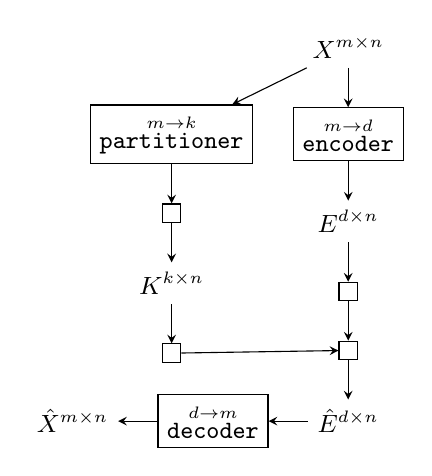
\begin{tikzpicture}[
    node distance = 5mm and 5mm,
    punkt/.style = {rectangle, draw},
    pil/.style = {black, -stealth},
    font=\small
    ]

  %\node[punkt] (preprocessing) {preprocessing} ;
  \node[] (X) {$X^{m \times n}$} ;
  \node[punkt] (encoder) [below=of X] {$\encoder^{m \to d}$} ;
  \node[] (E) [below=of encoder] {$E^{d \times n}$} ;
  \node[punkt] (Etranspose) [below=of E] {\transpose} ;

  \node[punkt] (partitioner) [left=of encoder] {$\partitioner^{m \to k}$} ;
  \node[punkt] (softmax) [below=of partitioner] {\softmax} ;

  \node[] (K) [below=of softmax] {$K^{k \times n}$} ;
  %\node[punkt] (Ktranspose) [left=of K] {\transpose} ;
  %\node[punkt] (KK) [below=of Ktranspose] {\matmul} ;
  %\node[] (P) [below=of KK] {$P^{n \times n}$} ;
  \node[punkt] (wak) [below=of K] {\PWAK} ;
  \node[punkt] (GE) [below=of Etranspose] {\matmul} ;
  \node[] (Ehat) [below=of GE] {$\hat{E}^{d \times n}$} ;

  \node[punkt] (decoder) [left=of Ehat] {$\decoder^{d \to m}$} ;
  \node[] (Xhat) [left=of decoder] {$\hat{X}^{m \times n}$} ;

  \draw[pil] %(preprocessing) edge (X)
  (X) edge (encoder)
  (encoder) edge (E)
  (E) edge (Etranspose)
  (Etranspose) edge (GE)
  
  (X) edge (partitioner)
  (partitioner) edge (softmax)
  (softmax) edge (K)
  (K) edge (wak)
  %(Ktranspose) edge (KK)
  %(K) edge (KK)
  %(KK) edge (P)
  %(P) edge (wak)
  (wak) edge (GE)
  (GE) edge (Ehat)

  (Ehat) edge (decoder)
  (decoder) edge (Xhat);
\end{tikzpicture}


         \caption{}
         \label{fig:}
     \end{subfigure}
     \hfill
     
     \caption{DeePWAK inference.
       See Appendix \ref{app:notation} for notation details.
     }
     \label{fig:deepwak}
\end{figure}

\paragraph{$\boxed{\times}$ Outer models}
\paragraph{$\boxed{\checkmark}$ DeePWAK flowchart}
Fig. \ref{fig:deepwak}
\paragraph{$\boxed{\times}$ PWAK example}
\paragraph{$\boxed{+}$ Diffusion example}
Take out DEWAKSS example. Substitute example from actual data.
\paragraph{$\boxed{+}$ Figure legends}

\subsubsection{Algorithms}
\paragraph{$\boxed{-}$ noise2self}
\paragraph{$\boxed{-}$ PWAK}

\subsection{Supplementary Publications}
\paragraph{$\boxed{\times}$ Theoretical foundations}
Material cut from \S \ref{sec:2}. Probably post to LessWrong.
\paragraph{$\boxed{+}$ DeePWAK}
Split out all microscopy and multihead stuff to
\url{https://drive.google.com/file/d/1geDArkvUQVOp79dF9knNmO3iP-1BYGOD/view?usp=drive_link}.

%\section{Methods}


\printbibliography

\appendix

\section*{Appendix} % Title for the entire appendix
\addcontentsline{toc}{section}{Appendix} % Optional: Add appendix title to the Table of Contents

%\begin{multicols}{2}
\section{Preliminary Results}
\secsubhead{I apologise for the information density of the figures.
I didn't have time to make simpler ones.}
\label{app:results}

\subsection{How to read the figures}
\label{sec:heatmaps}
%Heatmaps are ubiquitous in bioinformatics for visualizing very large data sets.
In Fig. \ref{fig:E_MNIST} and \ref{fig:K_MNIST}, rows are samples and columns are activations.
Samples are split either by training label (Fig. \ref{fig:E_MNIST}) or predicted label (Fig. \ref{fig:K_MNIST}.
Activations are split by model.
For Fig. \ref{fig:E_MNIST}, these are the encoder activations.
\textsf{bottleneck} gives the bottleneck activations for the outer model.
%\end{multicols}

\begin{figure}{\textwidth}
\centering
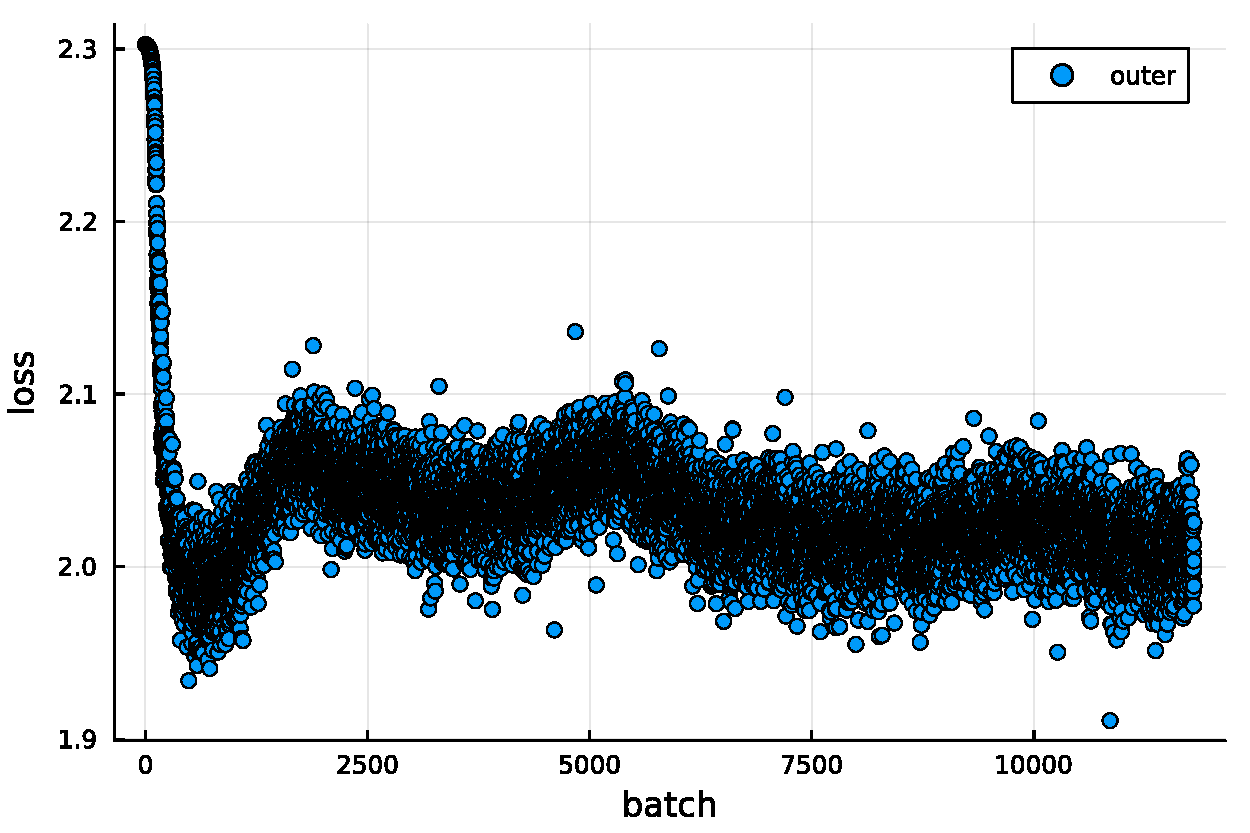
\includegraphics[width=\textwidth]{fig/loss_outer.pdf}
\caption{Outer model loss (logit crossentropy) compared to data labels.}
\label{fig:lossouter}
\end{figure}

\begin{figure}{\textwidth}
    \centering
    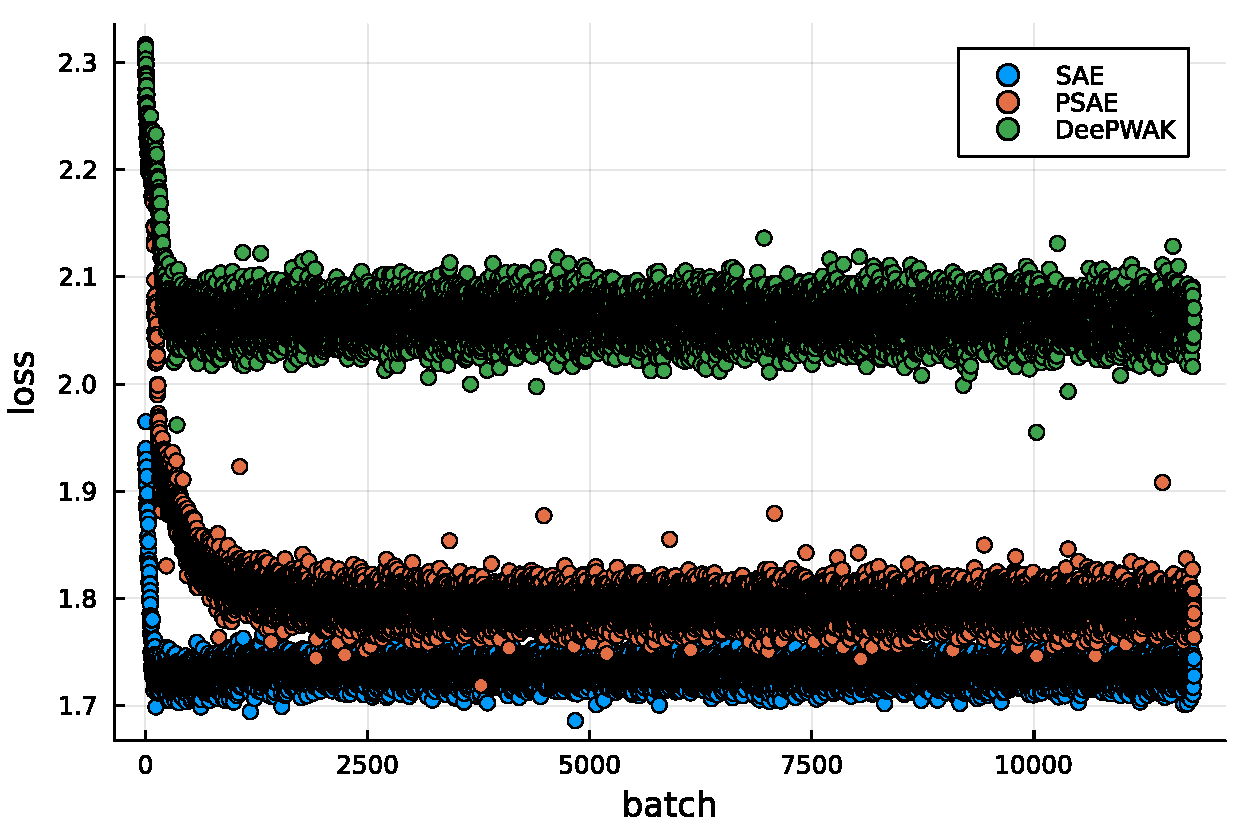
\includegraphics[width=\textwidth]{fig/loss_inner.pdf}
    \caption{Inner model loss (logit crossentropy) compared to the prediction of the outer model.}
    \label{fig:lossinner}
\end{figure}


\begin{figure}
  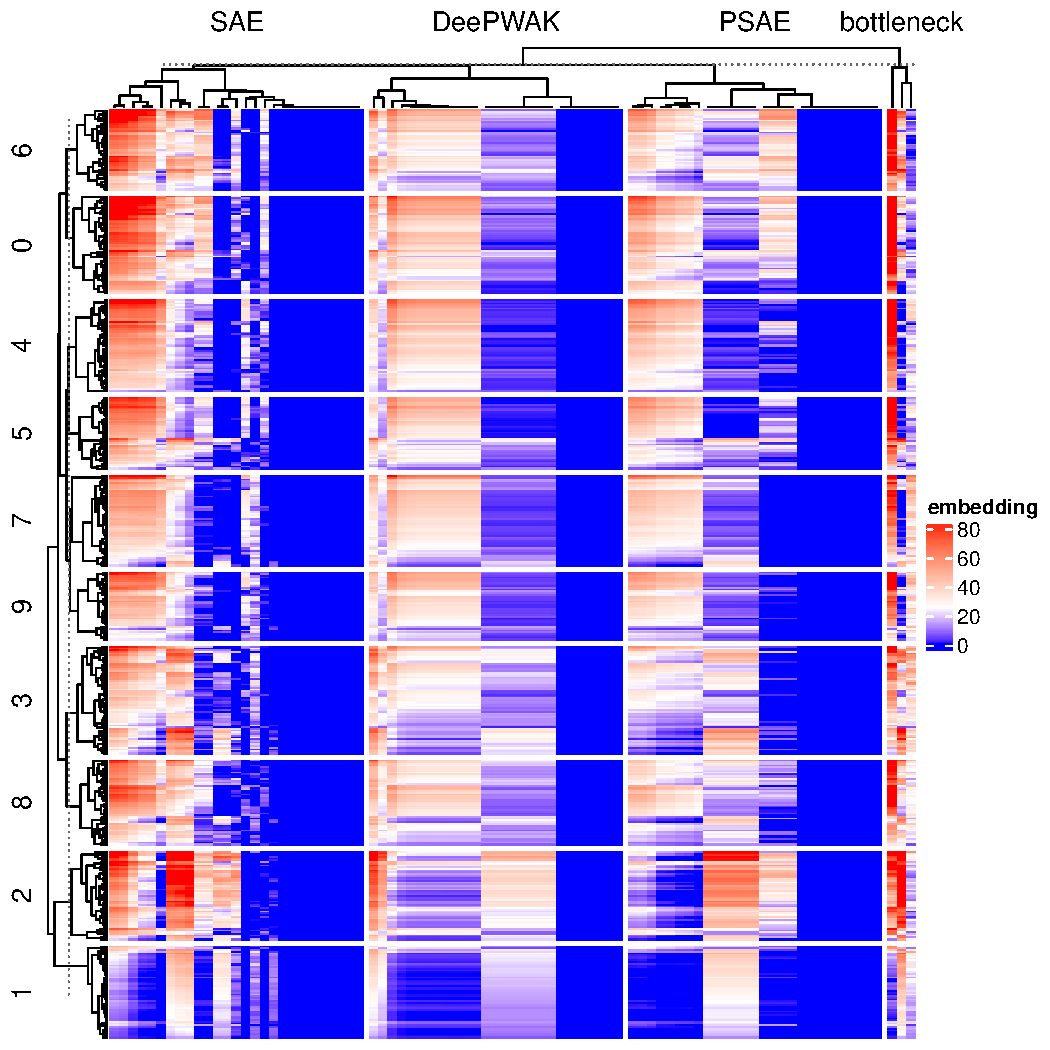
\includegraphics[width=\textwidth]{E_labels.pdf}
  \caption{Feature splitting of bottleneck activations by different methods.
    There is a clear progression of sparcity from a na\"ive SAE, PSAE, and DeePWAK.
    Rows are split by training set label.
    Interestingly, adding a partitioner submodel seems to result in the same feature being copied by multiple embeddings.}
    \label{fig:E_MNIST}
\end{figure}

\begin{figure}
  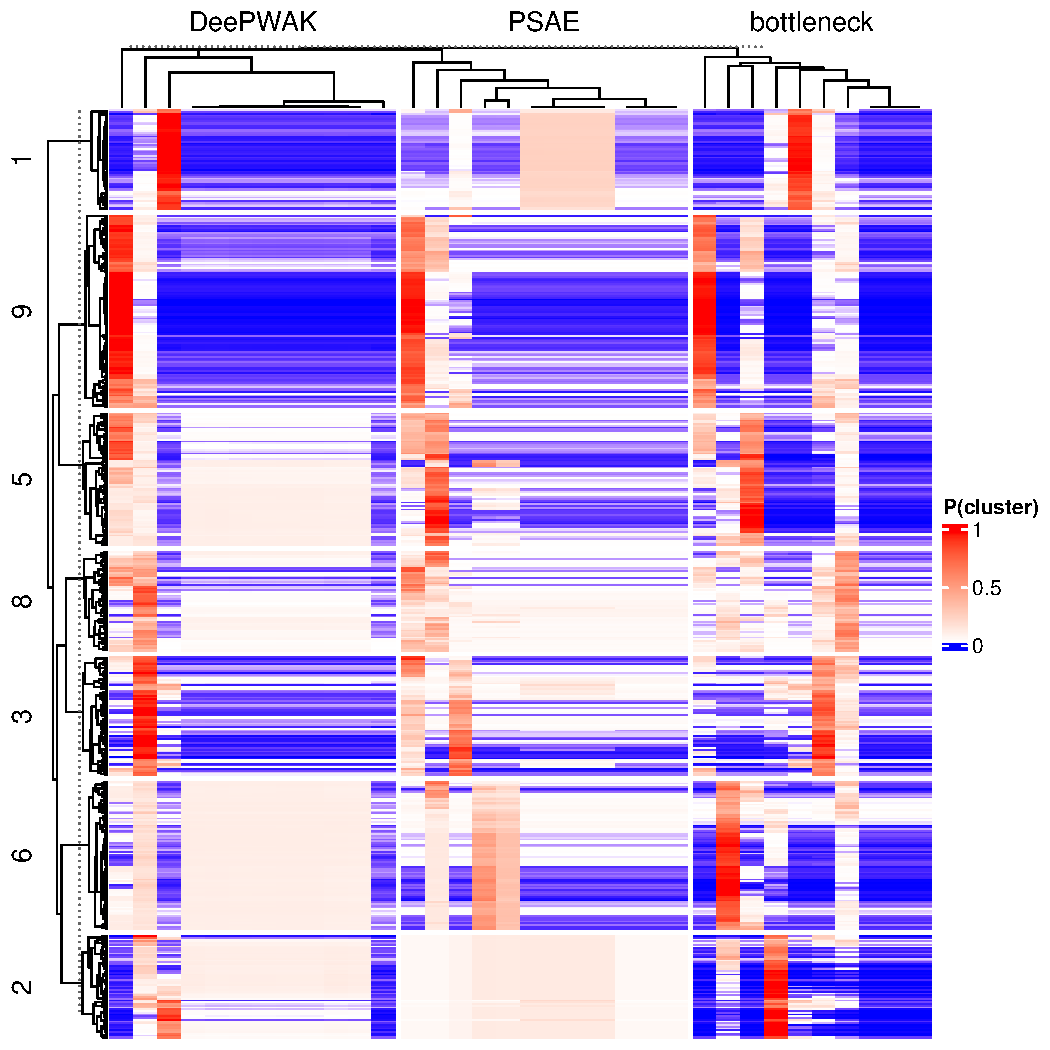
\includegraphics[width=\textwidth]{K_predicted.pdf}
    \caption{Both DeePWAK and PSEA learn sparse clusters. Rows are split by predicted label.}
    \label{fig:K_MNIST}
\end{figure}

\begin{figure}
  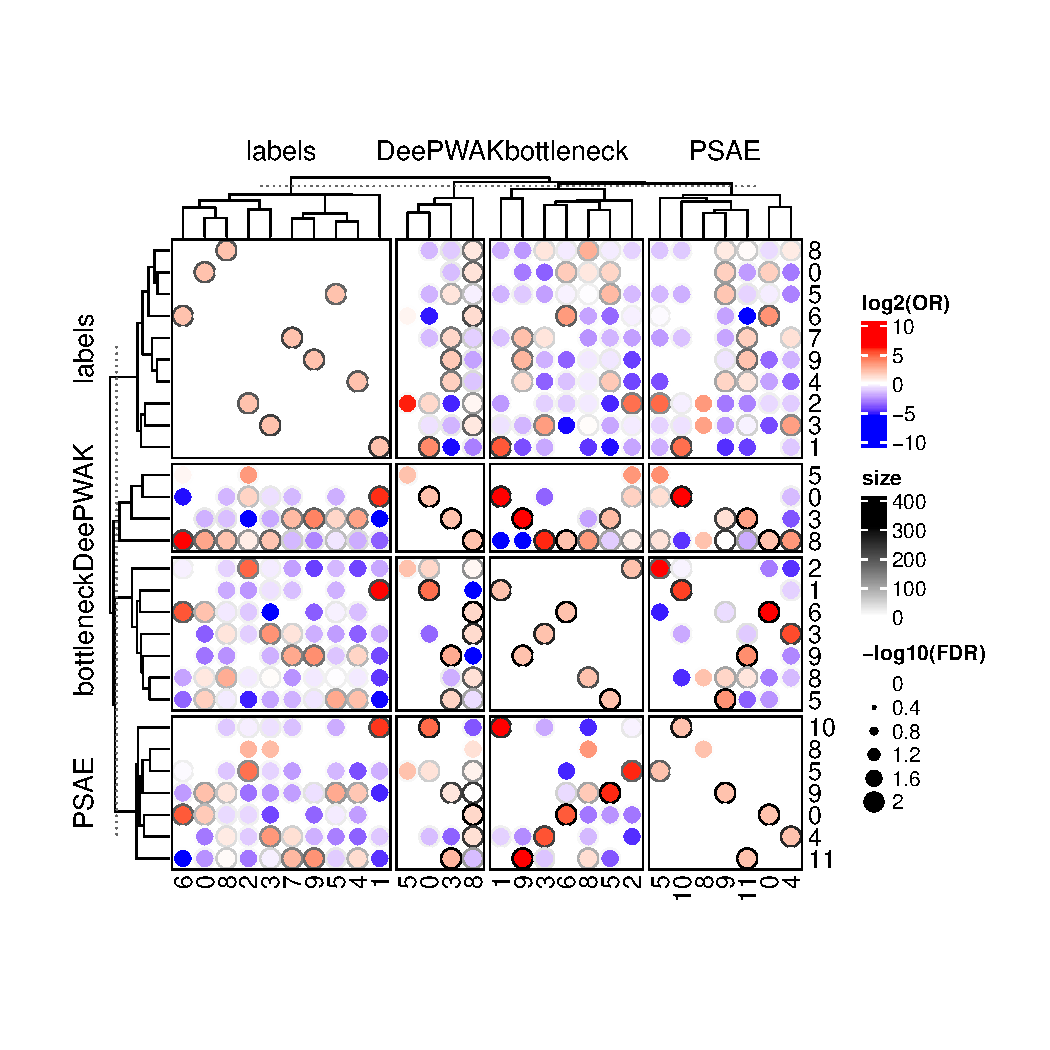
\includegraphics[width=\textwidth]{enrichment.pdf}
    \caption{Hypergeometric test for enrichment of [rows] in [columns].}
    \label{fig:hyperMNIST}
\end{figure}

%\begin{multicols}{2}
    
Even trained without a sparcity correction, \DeePWAK finds a more sparse representation than the SAE or PSAE (Fig. \ref{fig:E_MNIST}, \ref{fig:K_MNIST}.

Both DeePWAK and PSAE seem to capture latent features from the bottleneck (Fig. \ref{fig:hyperMNIST}.
Strikingly, PSAE better predicts the model output than the model predicts the training labels.
DeePWAK, on the other hand, appears to identify higher level features used by the model for classification.
It reveals the model apparently grouping rounded (0,3,6,8) and pointed (4,5,7,9) digits. 
Even more curiously, these features appear \textit{bisemantic}.
Looking at \textsf{DeePWAK 0}, this cluster appears to regard 6 as ``opposite'' of 1.
If we look back at Fig. \ref{fig:K_MNIST}, we can see the partitioner is much less confident classifying 6s than other digits.
It's possible the model is using an internal logic of ``I don't know what this is but it's definitely not a 1''.




\appendix

\section{Notation}
\label{app:notation}
We use lowecase Latin characters to denote scalars, boldface lowecase characters to denote vectors, and capital Latin characters to denote matrices.
Subscripts indicate indices.
Because we will mostly be working with matrices in $\mathbb{R}$, we abbreviate $X : \mathbb{R}^{m \times n}$ as $X^{m \times n}$.
We use a circumflex to indicate a reconstruction of an input by a predictor.
Lowercase Greek characters indicate the parameters of a model.
Capital Greek letters indicate parameter spaces.
Function names are in monospace.

$\fn^{n \to m}$ indicates a layer with input dimension $n$, output dimension $m$, and activation function $\fn$.

\section{Additional Background}
\label{app:bgd}

\subsection{Denoising the data explains the data}
\label{app:ntos}
For a large class of denoising functions, it is possible to find optimal parameters using only unlabeled noisy data\cite{batson2019noise2self}.
$\ntos$ gives a near-maximally-general optimization target for hyperparameter search.


Let $J \in \mathcal{J}$ be independent partitions of noisy data $X$.
Let $\mathcal{F}(\theta)$ be a family of predictors of $X_J$ with tunable parameters
$\theta \in \Theta$ that depends on its complement $X_{J^C}$

\begin{equation}
  \hat{X}_J=\mathcal{F}(\theta)(X_{J^C})
\end{equation}

In other words, $\mathcal{F}$ predicts each data point $X_J$ from some subset of the data excluding $X_J$. 

  The optimal $\theta$ is given by

\begin{equation}
  \label{eq:ntos}
  \ntos_\theta^{\Theta}[\mathcal{F}(\theta),X] := \argmin_\theta^{\Theta}[\sum_{J}^{\mathcal{J}}\mathbb{E}[X_J-\mathcal{F}(\theta)(X_{J^C})]^2]
\end{equation}

\subsection{Diffusion with weighted affinity kernels}

$\ntos$ is particularly useful for finding optimal parameters for generating a graph\cite{tjarnberg2021}.
(see Appendix \ref{app:DEWAKSS})
The adjacency matrix $G$ of any graph can be treated as a transition matrix (or weighted affinity kernel) by setting the diagonal to 0 and normalizing columns to sum to 1. We call this the \WAK function (Algorithm \ref{alg:WAK}).

For each value in data $X$, an estimate is calculated based on its neighbors in the graph. This can be expressed as matrix multiplication.

\begin{equation}
  \label{eq:WAK}
\hat{X} := \WAK(G)X^\top
\end{equation}


\subsection{Partitioned weighted affinity kernels} 
\label{app:pwak}

Though DEWAKSS uses a $k$-NN graph, any adjacency matrix will do.
A clustering can be expressed as a graph where points within a cluster are completely connected and clusters are disconnected.

Let $K^{k \times n}$ be a matrix representing a clustering of $n$ points into $k$ clusters. Let each column be a 1-hot encoding of a cluster assignment for each point. We can obtain a partition matrix $P \in \mathbb{R}^{n \times n}$ by what we'll call the \textit{partitioned weighted affinity kernel} (\PWAK) function.

\begin{equation}
  \label{eq:PWAK}
  \PWAK(K) := \WAK(K^\top K)
\end{equation}

This lets us define a loss function

\begin{equation}
  \mathcal{L}_{\mathPWAK}(K,X) := \mathbb{E}[\mathPWAK(K)X^\top - X]^2
\end{equation}


\PWAK can be extended to soft cluster assignment, making it possible to learn $K$ via SGD.
We will refer to a model of this sort as a \Partitioner to emphasize that while it returns logits corresponding to classifications, there are no labels on the training data.

There is no accuracy measure separate from the decoder loss.
The partitioner simply tries to find the best $P$ for minimizing loss of the decoded output.

The only hyperparameters are the maximum number of clusters, the neural net architecture, and the training hyperparameters.
Because $PX^\top$ is $\mathcal{J}$-invariant, this classifier will converge on a solution less than the maximum $k$.
Intuitions from transformers may be helpful in visualizing why this works.
Informally, $P$ can be equated to position-independent attention with data points as tokens and the batch size as the context window.
Attentive readers may make a connection between masking the diagonal and BERT.

We can now train a model to classify unlabeled data into an undefined number of clusters with no prior distribution in $\mathcal{O}(n^2)$ time!


\end{document}
